\documentclass{article}
\usepackage[utf8]{inputenc}
\usepackage{tikz,pgfplots}
\usetikzlibrary{positioning}
\usetikzlibrary {intersections}
\usetikzlibrary {shapes.symbols}
\usetikzlibrary{backgrounds}

% \title{TikZPrac}
% \author{Galaxy Being}
% \date{December 2022}

\begin{document}

%\maketitle


%\section{Introduction}

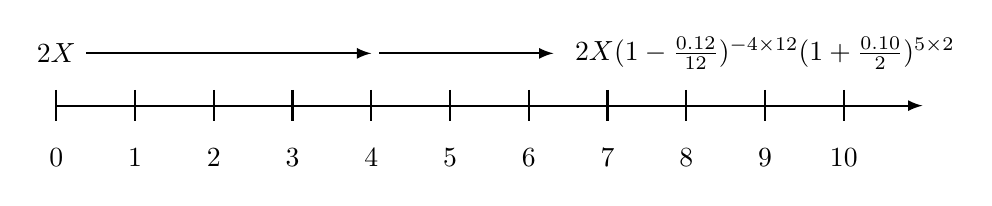
\begin{tikzpicture}[thick,time/.style={minimum height=5mm,minimum width=6mm,fill=#1,text=black},
  % every node/.style={draw},
  ]
  \draw[black,-latex] (0,0)--(11,0);
  \def\dx{1}
  \foreach \i in {0,...,10} {
    \ifnum\i>0
      \def\ann{$ $}
    \else
      \def\ann{$ 2X$}
    \fi
    \draw[] (\i*\dx,.2) -- (\i*\dx,-.2)
    node[pos=0,above=2mm,time=white] (P\i) {\ann}
    node[pos=1,below=2mm,time=white] (Q\i) {$\i$};
  }
  \node[time=white] at (P9) (x) {$2X(1-\frac{0.12}{12})^{-4\times12}(1+\frac{0.10}{2})^{5\times2} $};
  \draw[-latex] (P0)--(P4.center);
  \draw[-latex] ([xshift=1mm]P4.center)--(P6.east);
\end{tikzpicture}

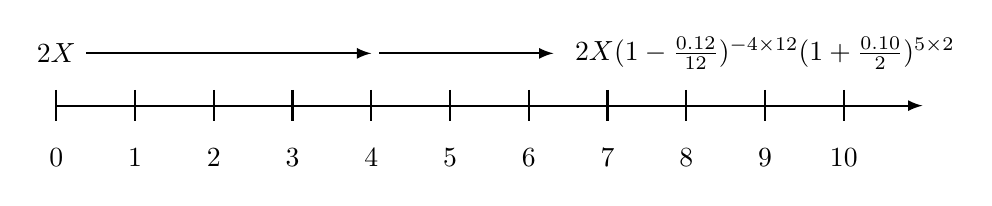
\begin{tikzpicture}[thick,time/.style={minimum height=5mm,minimum width=6mm,fill=#1,text=black},
  % every node/.style={draw},
  ]
  \draw[black,-latex] (0,0)--(11,0);
  \def\dx{1}
  \foreach \i in {0,...,10} {
    \ifnum\i>0
      \def\ann{$ $}
    \else
      \def\ann{$ 2X$}
    \fi
    \draw[] (\i*\dx,.2) -- (\i*\dx,-.2)
    node[pos=0,above=2mm,time=white,fill=none] (P\i) {\ann}
    node[pos=1,below=2mm,time=white,fill=none] (Q\i) {$\i$};
  }
  \node[time=white,fill=none] at (P9) (x) {$2X(1-\frac{0.12}{12})^{-4\times12}(1+\frac{0.10}{2})^{5\times2} $};
  \draw[-latex] (P0)--(P4.center);
  \draw[-latex] ([xshift=1mm]P4.center)--(P6.east);
\end{tikzpicture}


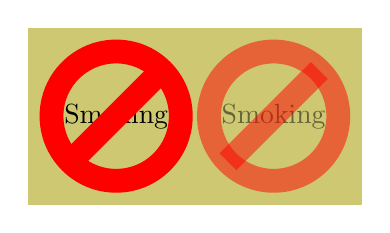
\begin{tikzpicture}[background rectangle/.style={fill=olive!45}, show background rectangle]
  \node at (0,0) [forbidden sign,line width=2ex,draw=red,fill=none] {Smoking};

  \node [opacity=.5]
        at (2,0) [forbidden sign,line width=2ex,draw=red,fill=none] {Smoking};
\end{tikzpicture}





\end{document}